\documentclass[../Bachelorarbeit.tex]{subfiles}

\begin{document}
The EFT samples for each parameter S0, M0, M1, T0, T1, T2 is fitted against the combined SM and GM Resonance data. It is assumed that the coefficients are only affected by aQCD couplings.
Only one coefficient is fitted while the other coefficients are set to zero. As discussed in section \ref{sec:EFT} good fits are expected for sufficiently high resonance mass.
The fit can't identify small energies or high energy with small cross-sections resonances as shown in \ref{fig:S1_with_fit_diffrence_225}.

\begin{figure}[h]
    \centering
    \begin{subfigure}{0.3\textwidth}
        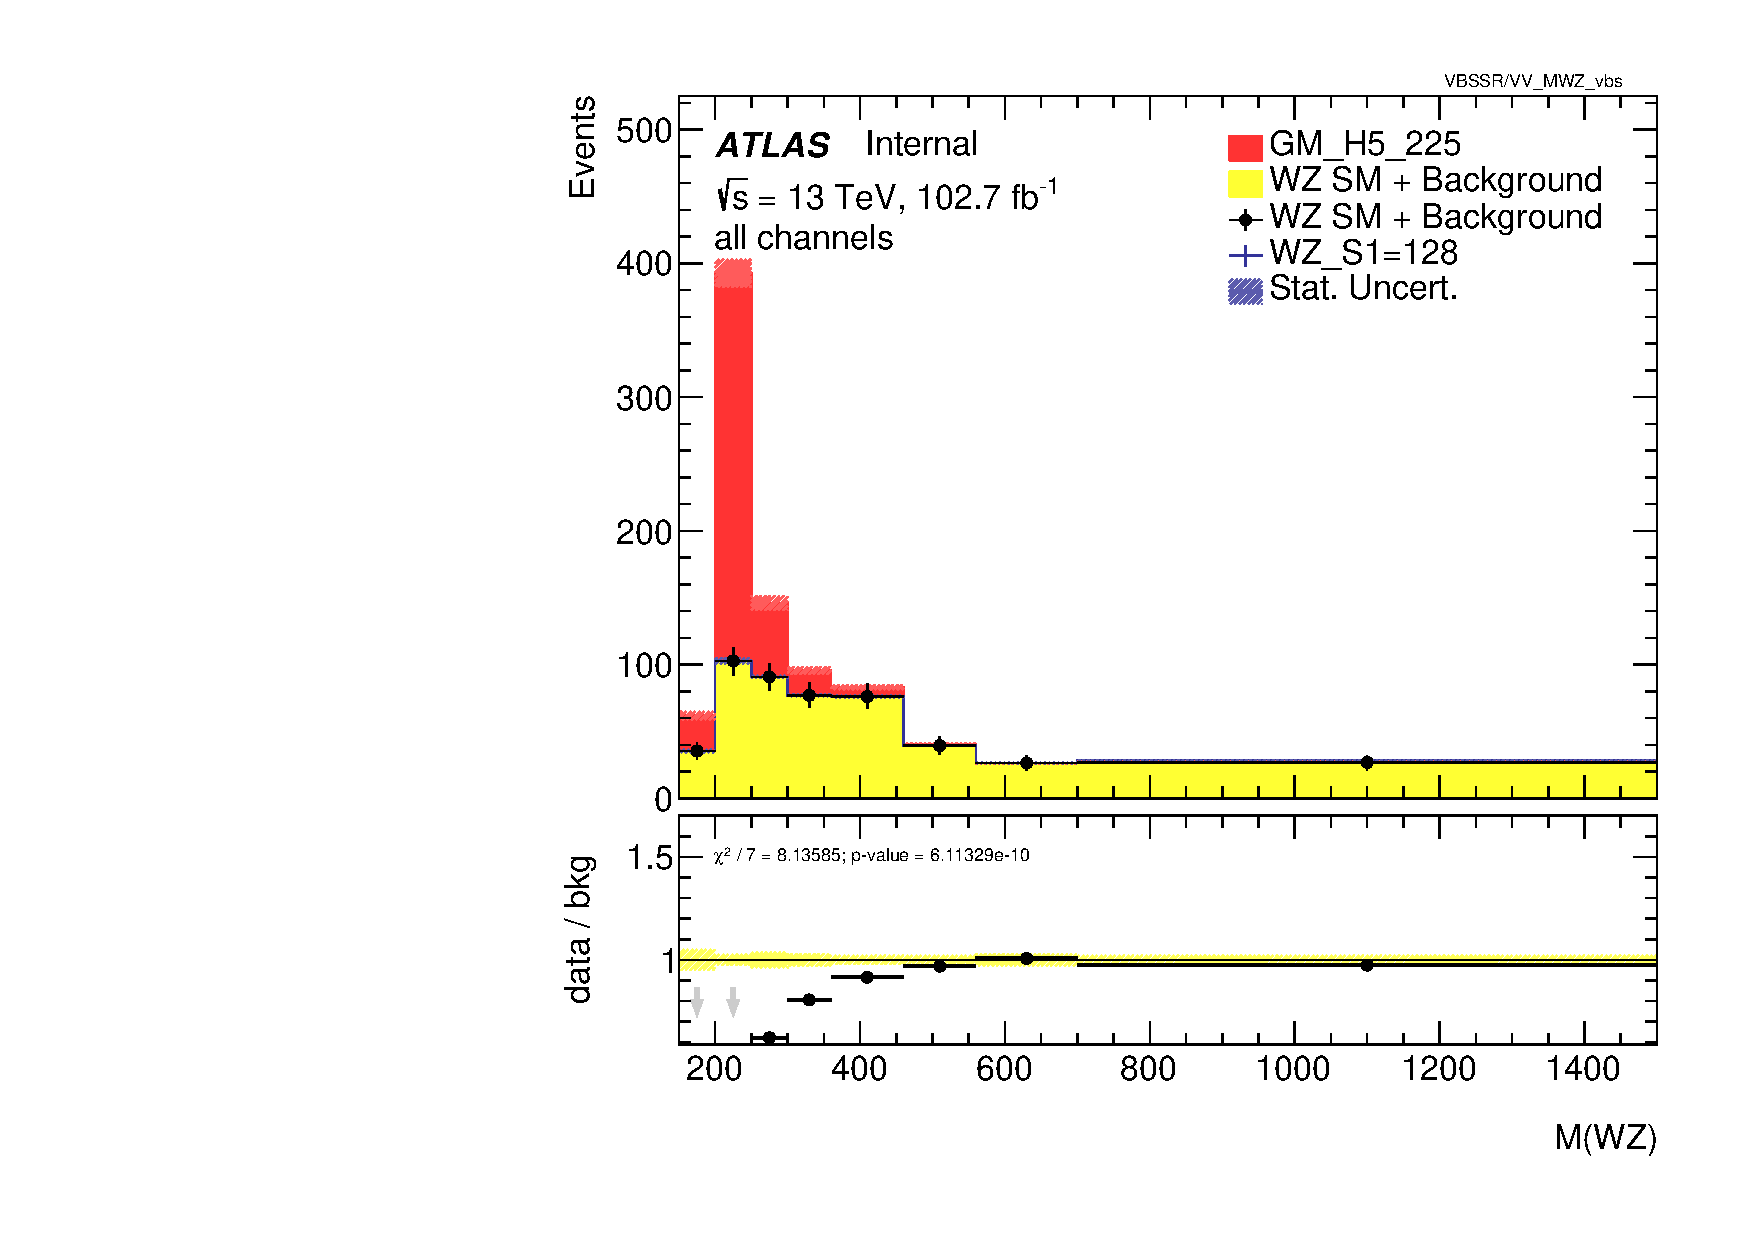
\includegraphics[width=\textwidth]{Plots/operators/all_VV_MTWZ_vbs_225.pdf}
        \caption{}
    \end{subfigure}
    \begin{subfigure}{0.3\textwidth}
        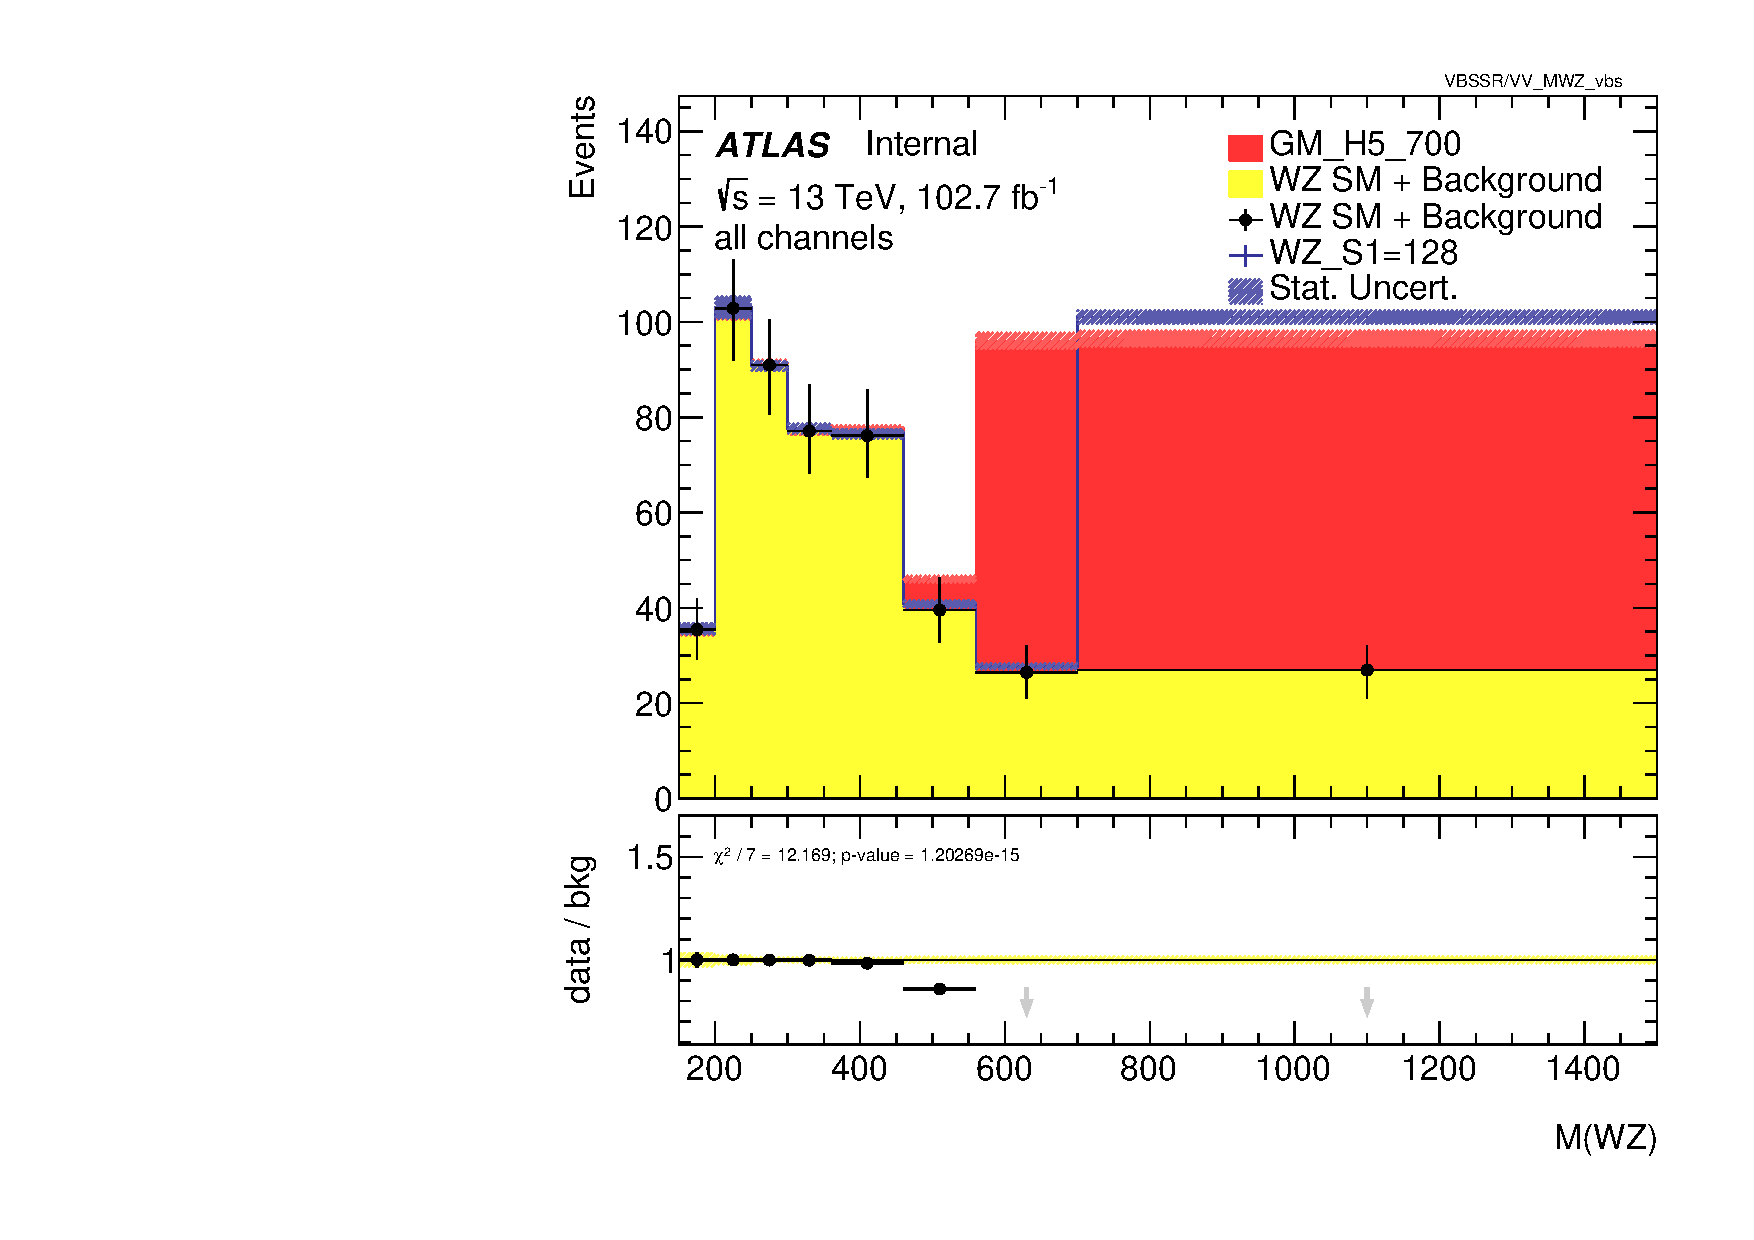
\includegraphics[width=\textwidth]{Plots/operators/all_VV_MTWZ_vbs_700.pdf}
        \caption{}
    \end{subfigure}
    \begin{subfigure}{0.3\textwidth}
        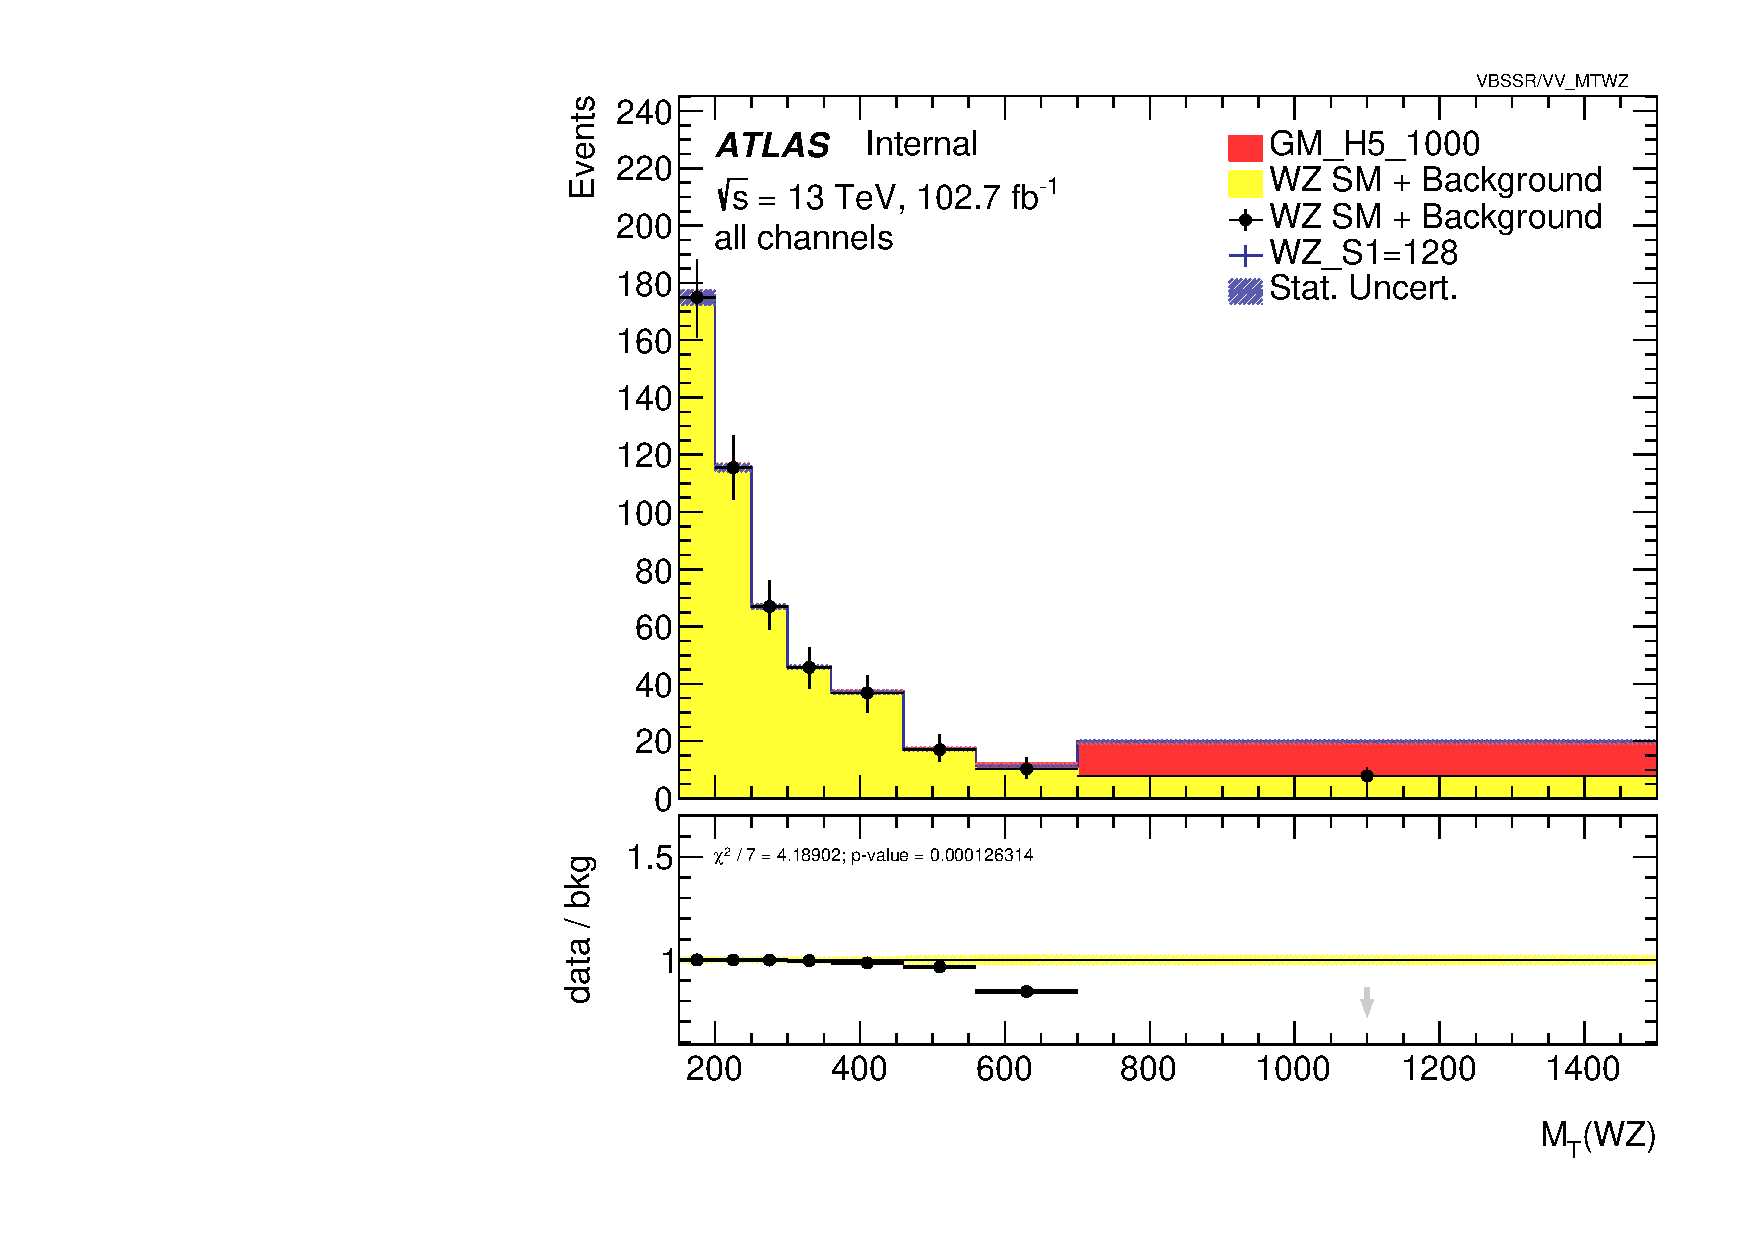
\includegraphics[width=\textwidth]{Plots/operators/all_VV_MTWZ_1000.pdf}
        \caption{}
    \end{subfigure}
    \caption{\textbf{a)}The invariant Mass of the resonance has approximately the same energy as the WZ peak but for the WZ peak the EFT prediction
        should be the SM therefore EFT can't describe the 225 GeV Resonance and the coefficient fit diverges.
        \textbf{b)}700 GeV has a high cross-section and the energy is in the region where SM and EFT deviate therefore the coefficients can be fitted accurately.
        \textbf{c)}1000 GeV the cross-section is to low the fit can produce a significant result even though the Resonance is in the right Energy region.}
    \label{fig:S1_with_fit_diffrence_225}
\end{figure}

Evaluating which fit is good can be done qualitative by simply looking at the invariant Mass plots if the EFT Sample scaled with the best fit value is able to describe
the Resonance one can argue that the fit is good. But this is not accurately possible for resonances peaks that are higher energy than the WZ peak, but the start of the peak is still part of the WZ peak.
For a quantitative analysis the significants quotient has to be calculated from the log-likelehood function $f(x)=-2\Delta log(L)$.
The significants can be calculate using $Z(x)=\sqrt{f(x)}$ resulting in $S = \frac{Z_{GM}(0)}{Z_{EFT}(0)}$.
Here $Z_{GM}$ is the significants when the GM Sample is used as coefficient in EFT-Fun and fitted with SM as measurement and as prediction.
The $Z_{EFT}$ is the fit of an EFT coefficient for the SM combined with the GM Model as measurement against the SM as prediction.
$f(0)$ can be interpreted as the difference to the SM, if $f(0) = 0$ only the SM was measured and for $f(0) > 0$ the SM is excluded.
The value of $f(0)$ can be read off from the likelehood-funktion in \ref{fig:EFT_GM_Asimov_comparision}. The scale is dependent on
the operator as well as the allowed range making it difficult to estimate a read off error. The error can be minimized by looking at positive and negative extrema and limiting the range to zero as well as the shape including both extrema.
Since the likelihood-function continuous all plots give the same $f(0)$ value. All three ranges should be used in case only an extremum exists, or only one is recognized by the fit this is often the case for low resonace energies.
Using this the error becomes small compared to the statistical errors. 



\begin{figure}[h]
    \centering
    \begin{subfigure}{0.3\textwidth}
        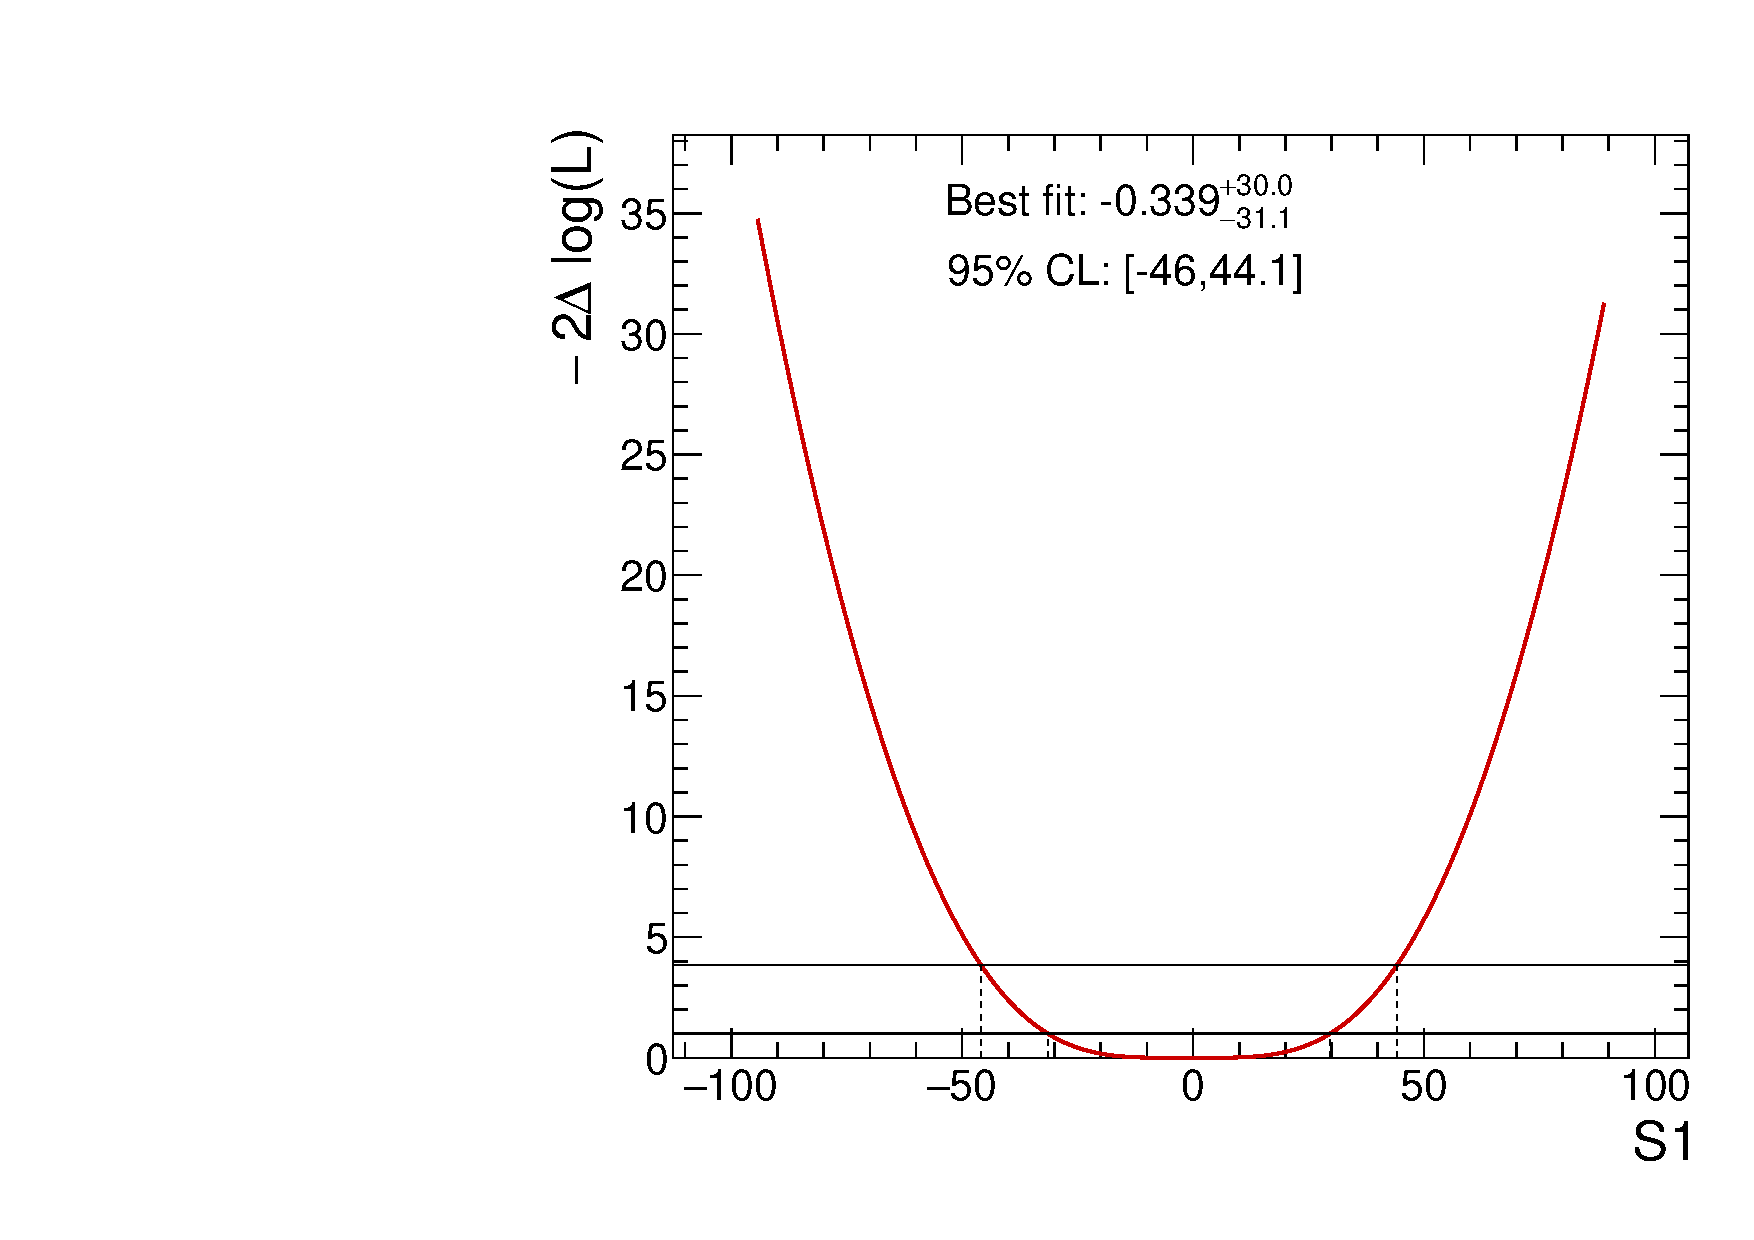
\includegraphics[width=\textwidth]{Plots/operators/S1_asimov.pdf}
        \caption{S1 Asmiov fit}
    \end{subfigure}
    \begin{subfigure}{0.3\textwidth}
        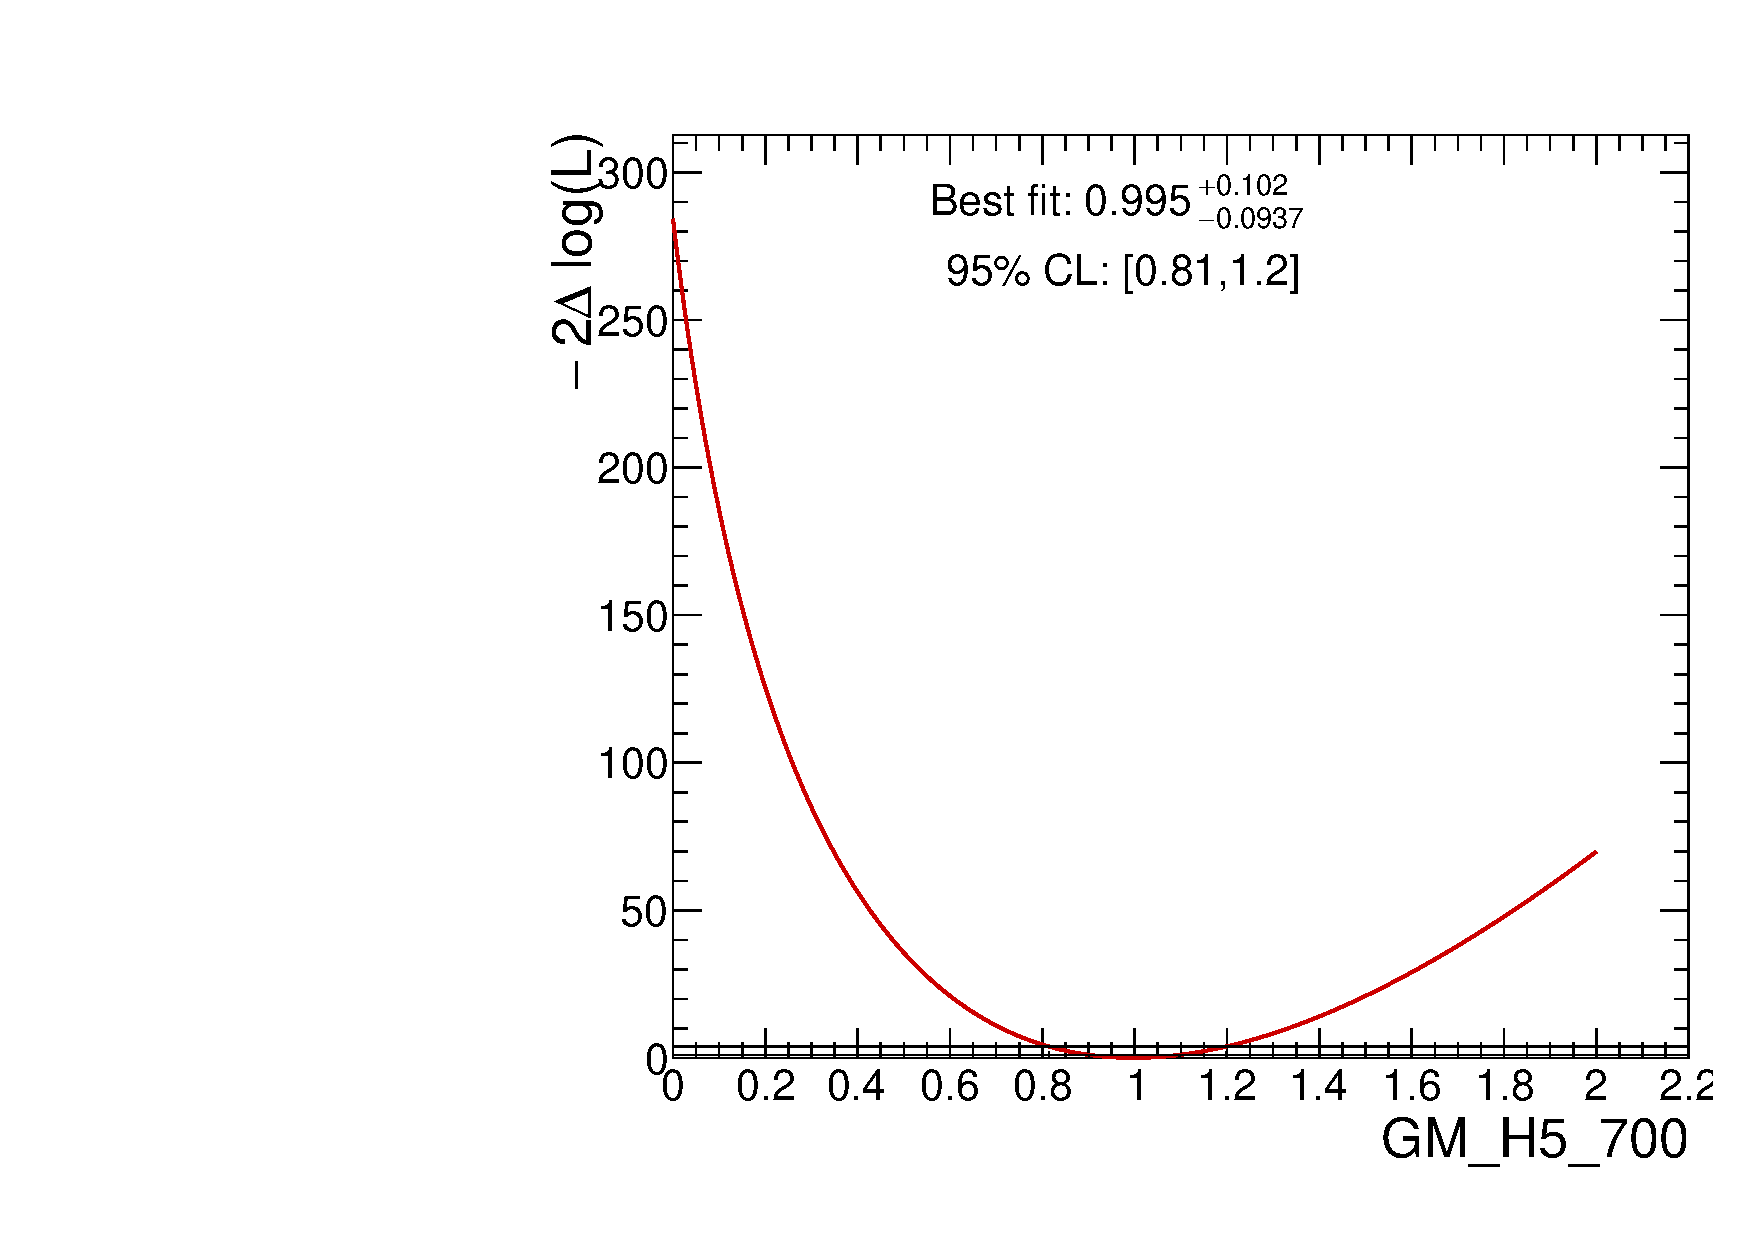
\includegraphics[width=\textwidth]{Plots/operators/GM_H5_700_scan_coef.pdf}
        \caption{700 GeV GM}
    \end{subfigure}
    \begin{subfigure}{0.3\textwidth}
        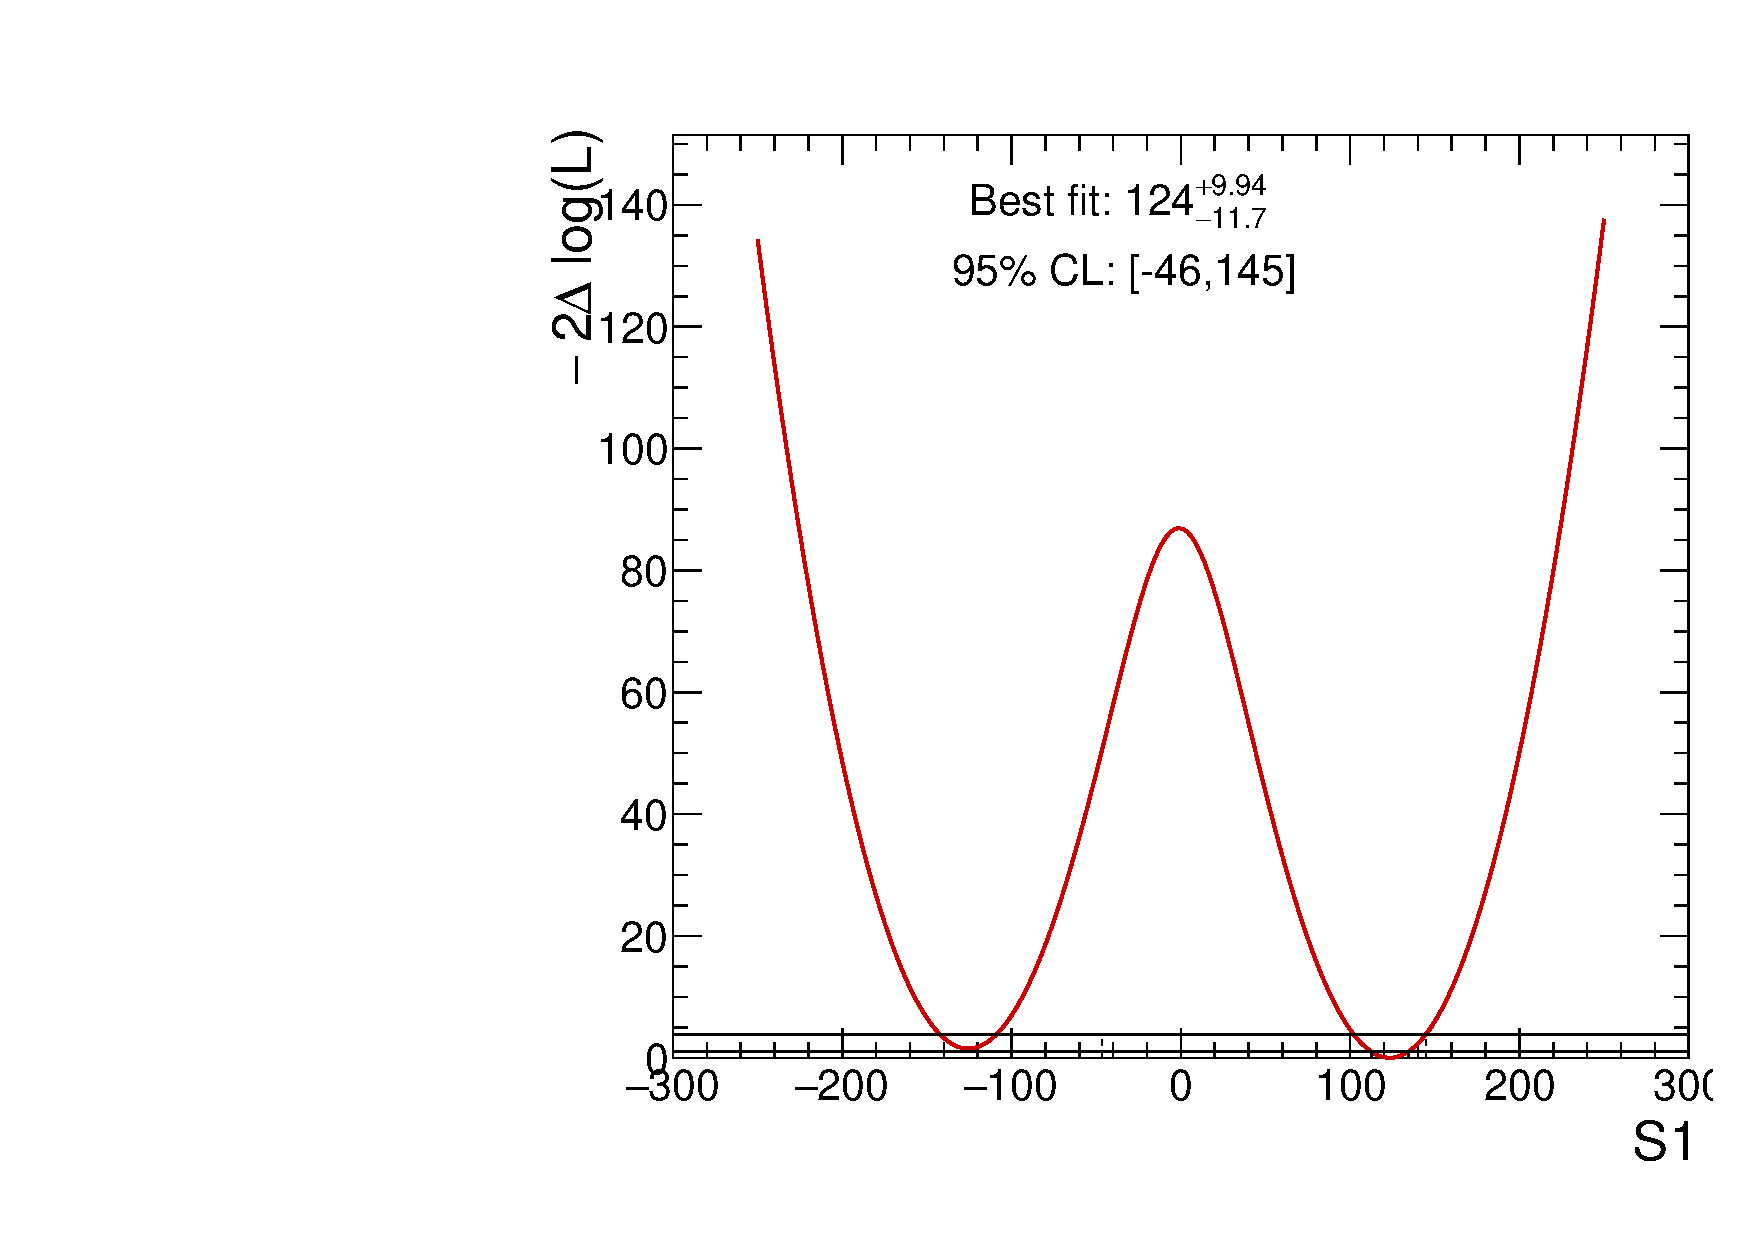
\includegraphics[width=\textwidth]{Plots/operators/S1_EFT.pdf}
        \caption{S1 for 700 GeV}
    \end{subfigure}
    \caption{\textbf{a)}The best fit value is zero since the SM is reproduced in the asimov fit.
    \textbf{c)} The SM is exluded an two extrma emerge from the inclusion of the quadratic operator therm.}
    \label{fig:EFT_GM_Asimov_comparision}
\end{figure}

\begin{figure}
    \centering
    \begin{subfigure}{0.45\textwidth}
        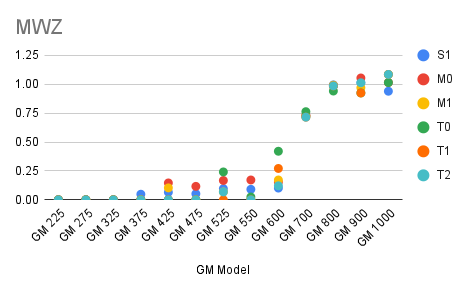
\includegraphics[width=\textwidth]{Plots/significans/MWZ.png}
        \caption{}
    \end{subfigure}
    \begin{subfigure}{0.45\textwidth}
        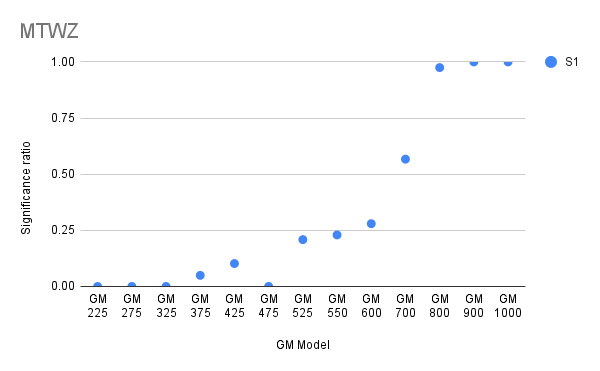
\includegraphics[width=\textwidth]{Plots/significans/MTWZ.png}
        \caption{}
    \end{subfigure}
    \caption{}
    \label{fig:significans_plots}
\end{figure}
\end{document}